\section[Bonus Item]{Bonus Item : Real-time''}
\begin{frame}{PSF estimation}

The angle and length estimation are achieved with a $256 \times 256 $ pixels square. 
 
\begin{figure}[h]
\centering
\begin{subfigure}{0.4\textwidth}
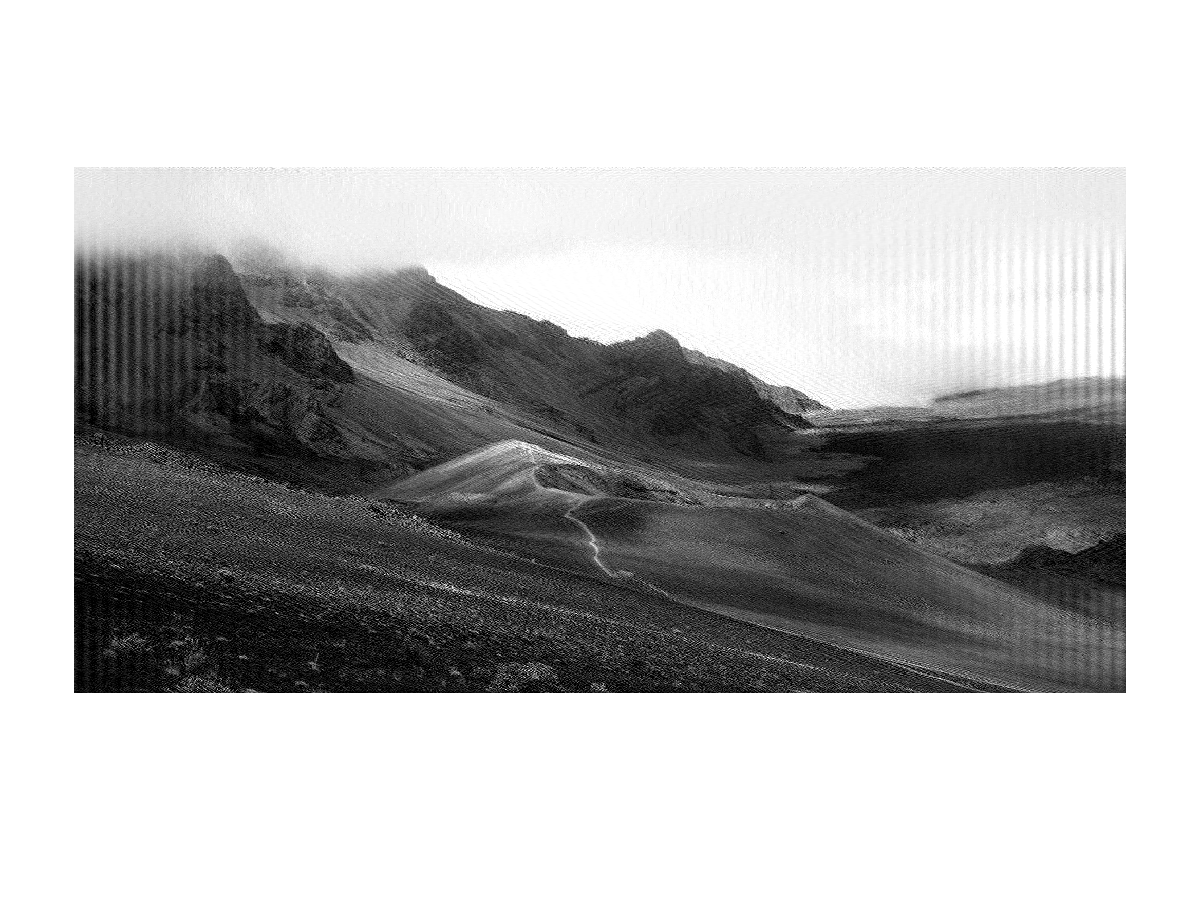
\includegraphics[width= \textwidth]{../Images/SagarShortEstimation.png}
\vspace{-20pt}
\caption{ $256\times 256$ centered crop of the picture. }
\label{fig:SagarShort}
\end{subfigure}
~
\begin{subfigure}{0.4\textwidth}
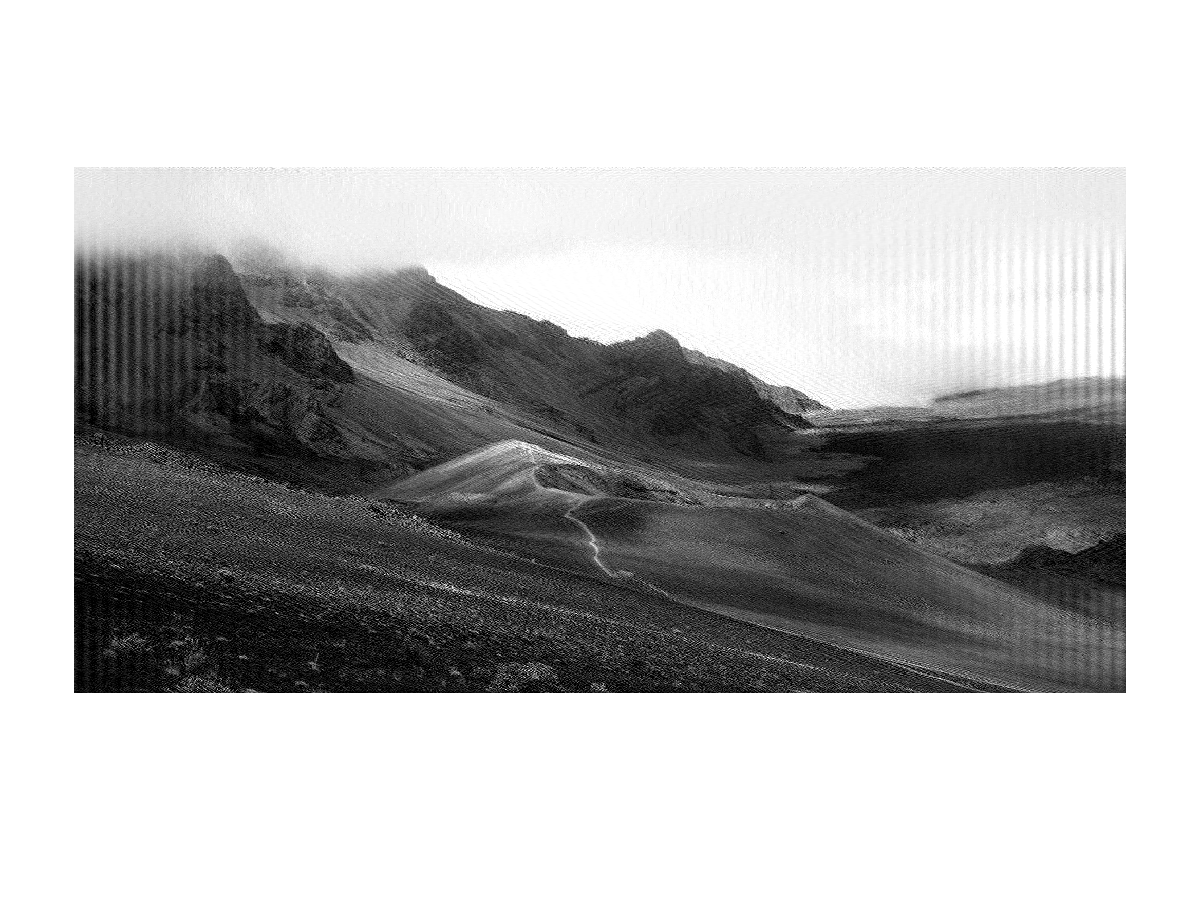
\includegraphics[{width= \textwidth}]{../Images/SagarLongEstimation.png}
\vspace{-20pt}
\caption{The whole image.}
\label{fig:SagarLong}
\end{subfigure}
\caption{Different matrix's size for the PSF estimation.}
\end{figure}
\end{frame}

\begin{frame}{Resizing}
 
Challenge : Artifacts may occur during the resizing process. 

\begin{figure}
\centering
\begin{subfigure}{0.4\textwidth}
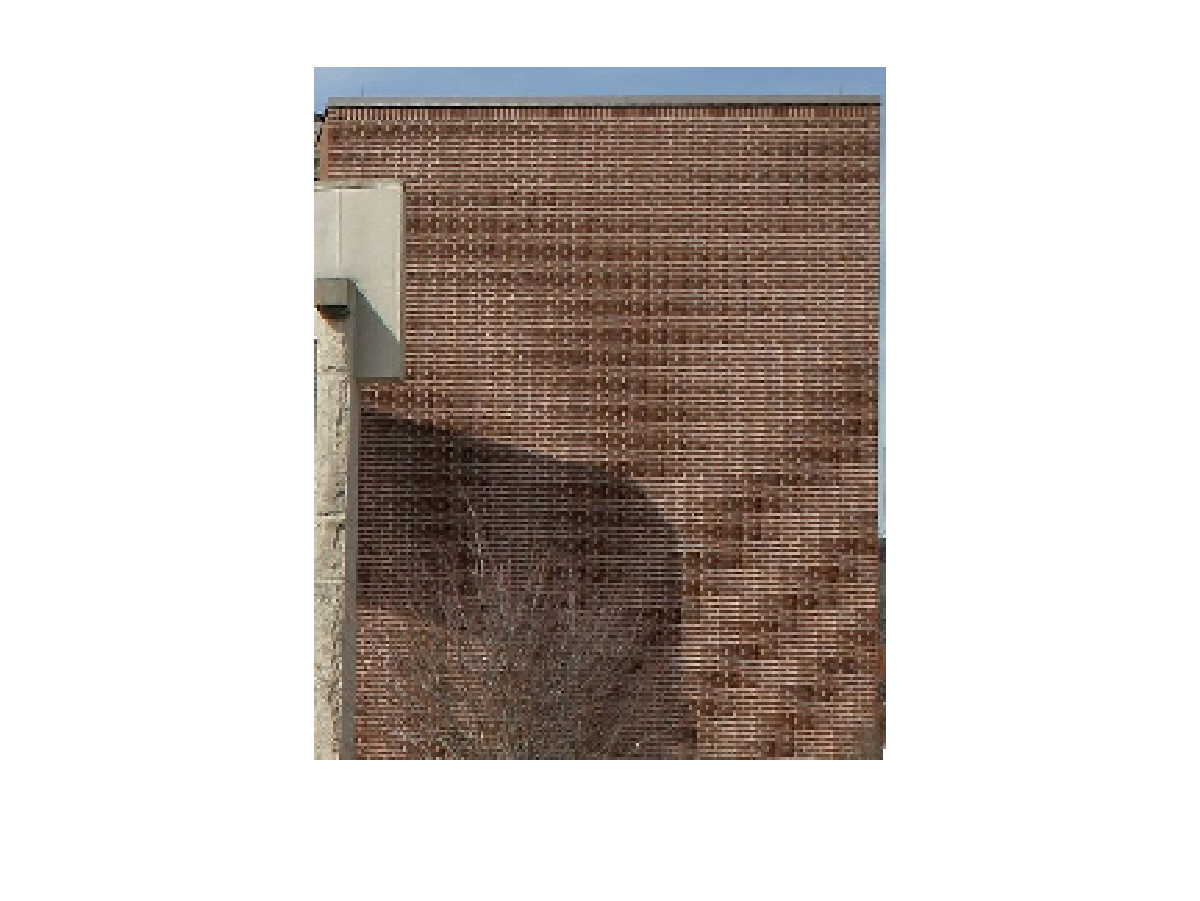
\includegraphics[width= \textwidth]{../Images/bricksCompressed.png}
\vspace{-20pt}
\caption{Nearest-Neighbor algorithm. }
\label{fig:bricksCompressed}
\end{subfigure}
~
\begin{subfigure}{0.4\textwidth}
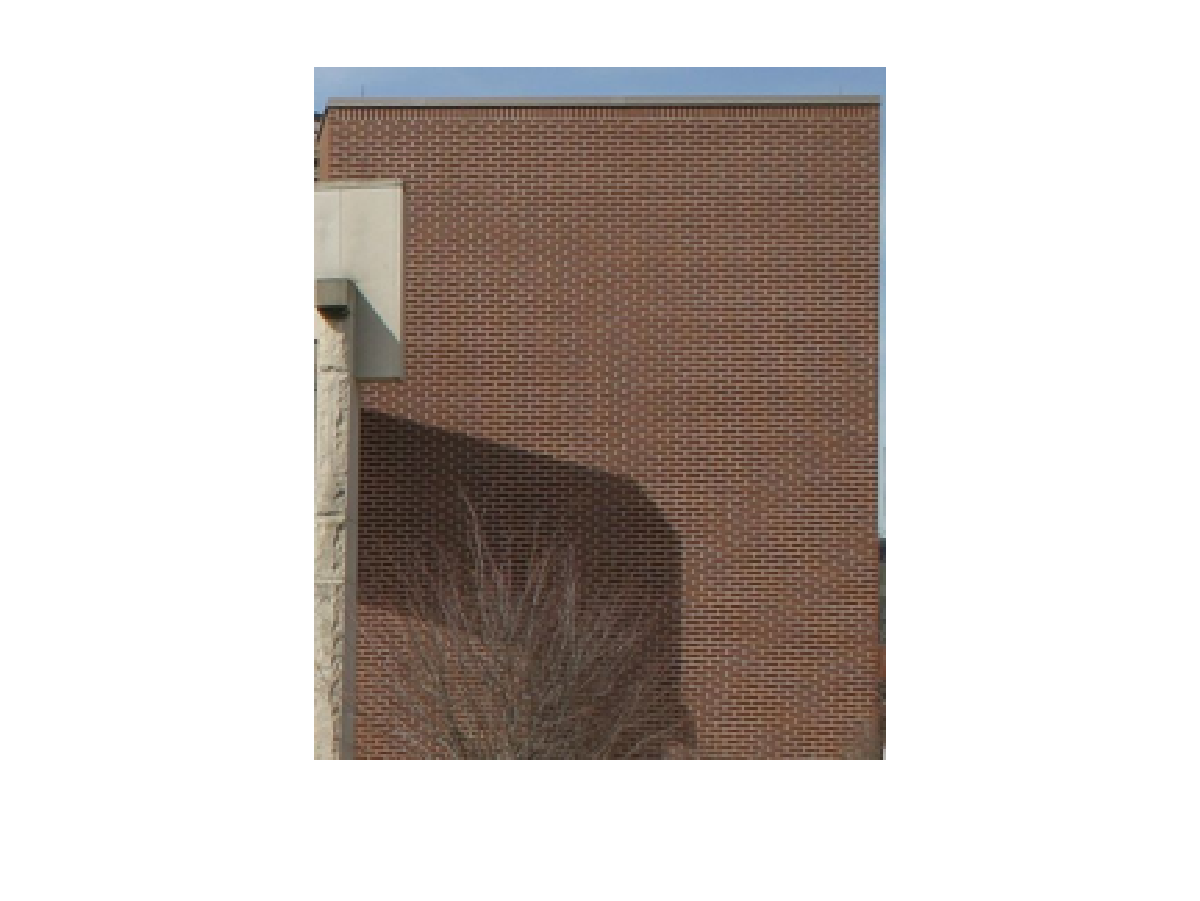
\includegraphics[width = \textwidth]{../Images/bricksLanczos.png}
\vspace{-20pt}
\caption{Lanczos2 algorithm.}
\label{fig:bricksLanczos}
\end{subfigure}
\caption{Picture resized using different algorithms}
\end{figure}

\end{frame}
